% TEMPLATE for Usenix papers, specifically to meet requirements of
%  USENIX '05
% originally a template for producing IEEE-format articles using LaTeX.
%   written by Matthew Ward, CS Department, Worcester Polytechnic Institute.
% adapted by David Beazley for his excellent SWIG paper in Proceedings,
%   Tcl 96
% turned into a smartass generic template by De Clarke, with thanks to
%   both the above pioneers
% use at your own risk.  Complaints to /dev/null.
% make it two column with no page numbering, default is 10 point

% Munged by Fred Douglis <douglis@research.att.com> 10/97 to separate
% the .sty file from the LaTeX source template, so that people can
% more easily include the .sty file into an existing document.  Also
% changed to more closely follow the style guidelines as represented
% by the Word sample file. 

% Note that since 2010, USENIX does not require endnotes. If you want
% foot of page notes, don't include the endnotes package in the 
% usepackage command, below.

% This version uses the latex2e styles, not the very ancient 2.09 stuff.
\documentclass[letterpaper,twocolumn,10pt]{article}
\usepackage{usenix,epsfig,endnotes}
\begin{document}

%don't want date printed
\date{}

%make title bold and 14 pt font (Latex default is non-bold, 16 pt)
\title{\Large \bf Android Low Entropy Demystified}

%for single author (just remove % characters)
\author{
{\rm Yuanyuan Zhou}\\
University of Michigan, Ann Arbor
\and
{\rm Zhuo Peng}\\
University of Michigan, Ann Arbor
% copy the following lines to add more authors
% \and
% {\rm Name}\\
%Name Institution
} % end author

\maketitle

% Use the following at camera-ready time to suppress page numbers.
% Comment it out when you first submit the paper for review.
%\thispagestyle{empty}


\subsection*{Abstract}
We look into the issue that the amount of entropy kept by the pseudorandom number generator (PRNG) of Android is constantly low. We find that the accusation against this issue of causing poor performance and low frame rate experienced by users is ungrounded. We also investigate possible security vulnerabilities resulting from this issue. We find that this issue does not affect the quality of random numbers that are generated by the PRNG and used in Android applications because recent Android devices do not lack entropy sources. However, we identify a vulnerability in which the stack canary for all future Android applications is generated earlier than the PRNG is properly setup. This vulnerbility makes stack overflow simpler and threats Android applications linked with native code (through NDK) as well as Dalvik VM instances. An attacker could nullify the stack protecting mechanism, given the knowledge of the time of boot or a malicious app running on the victim device. This vulnerability also affects the address space layout randomization (ALSR) mechanism on Android, and can turn it from a weak protection to void. We discuss in this paper several possiable attacks against this vulnerbility as well as ways of defending. As this vulnerbility is rooted in an essential Android design choice since the very first beginning, it is difficult to fix.



\section{Introduction}
\subsection{Motivation}

Our motivation roots in an issue reported to the Android Open Source Program \cite{issue42265} , which complained about the constantly low amount of entropy kept by the PRNG affected the overall performance and user experience, causing low frame rate in the UI layer. There was a solution proposed by the XDA community which periodically wrote into \verb|/dev/random|. The idea behind the solution is that the lag is attributed to the blocking read of \verb|/dev/random|; writing into \verb|/dev/random| raises the amount of entropy and processes blocking on \verb|/dev/random| then get unblocked. 

We first want to investigate whether this accusation is grounded and whether the solution does any help, since the solution, as described by some users, resolved the long-lived lagging UI issue of Android.

Furthermore, this issue reminds us the identical or factorable RSA private keys vulnerability prevalent among embedded devices which lack sources of entropy and have constantly low amount of entropy \cite{weakkeys12}. We want to know if there is a similar vulnerability on the Android devices, which could also lack entropy sources during boot, especially during their first boot: the applications which require high quality random numbers, such as a disk encryption application,  get predictable or identical results from the PRNG.

\subsection{Linux PRNG and Our Assumption}
Android runs on a Linux kernel. The \verb|/dev/random| and \verb|/dev/urandom| devices are backed by the Linux PRNG. Figure \ref{figprng} shows its general structure \cite{Gutterman06}. In this section, we briefly describe how it works and its properties related to our work.

\begin{figure}[t]
\begin{center}
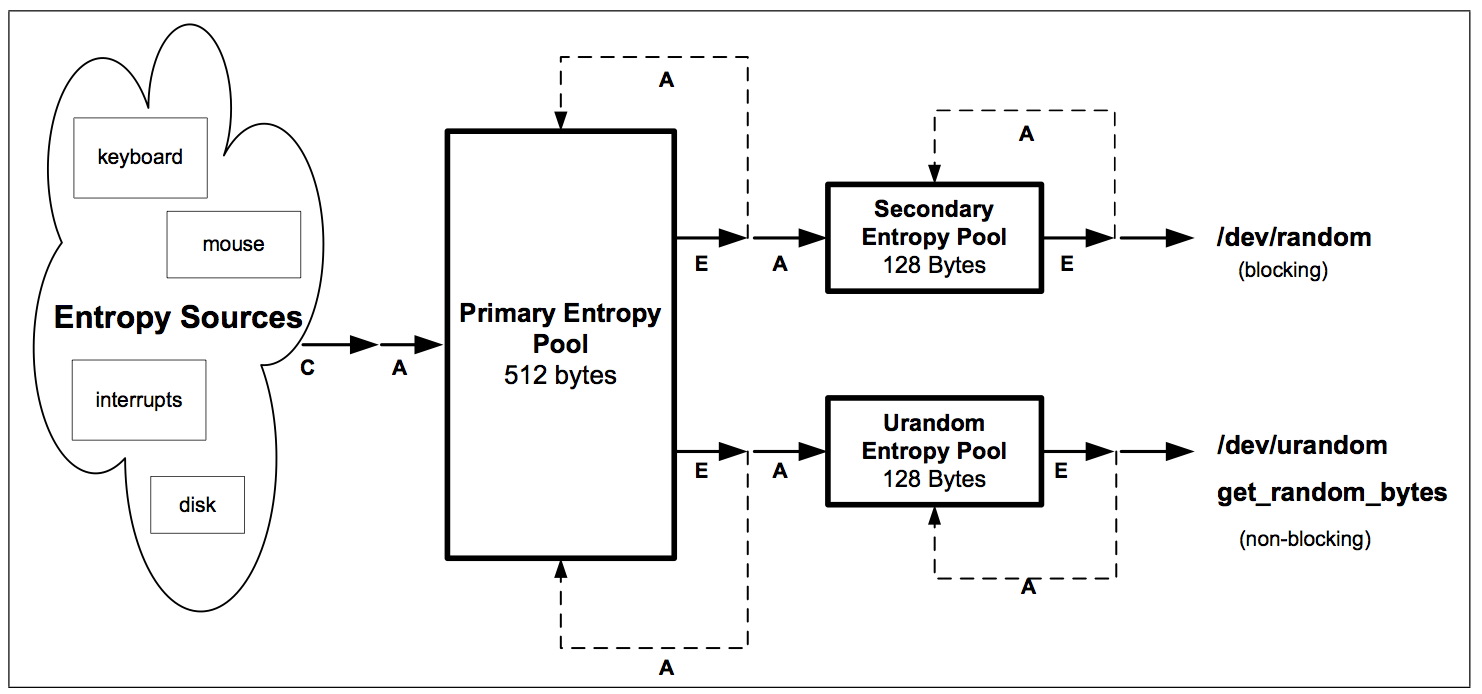
\includegraphics[scale=0.27]{prng.png}
\end{center}
\caption{{\bf General Structure of Linux PRNG}}
\label{figprng}
\end{figure}


The Linux PRNG consists of three entropy pools which act in a same manner. They have two major functions: mix entropy into the pool and extract entropy from the pool. The input pool (also known as the primary pool) gets entropy from three types of entropy sources: disk, interrupt and input events. When an event happens in a source, the source feeds the timing and the type of the event to the input pool. The two output pools (secondary pools) get their entropy by extracting entropy from the input pool. The blocking pool blocks upon no entropy in both its pool and the input pool while the non-blocking pool does not. An important property of the non-blocking pool is that it does not extract any entropy if the amount of entropy in the input pool is less than 192 (\verb|random_read_wakeup_thresh * 3 / 8|) bits. When there is no entropy mixed into the non-blocking pool, its output is deterministic and predictable given any of its internal states between the last entropy mix and the number of extractions from it. 

The three pools are initialized when the kernel initializes the random character device. On initialization, the pools are not wiped and the time and machine information are mixed in. Under traditional Linux environment, there is an init script which reads the saved random seed from the disk and mixes it into the nonblocking pool.

Our assumption on Linux PRNG is the following: after the first time when \verb|/dev/urandom| extracts enough entropy (for example, the minimum amount of extraction, 60 bits) from the input pool, \verb|/dev/urandom| is secure. It makes no difference that the amount of entropy is low or high after this time point.


The rest of the paper is organized as follows. In section 2, we introduce existing work on analyzing Linux PRNG and the low entropy issue, as well as the work aiming at exploiting or defending buffer overflow. Section 3 describes our investigation methodology. Section 4 shows the result of our investigation, revealing several vulnerabilities. In Section 5 we discuss the effect of these vulnerabilities and possible attacks and defenses. Finally, in section 6 we draw our conclusion.


\section{Related Work}


Previous work was done to analysis the security of the Linux PRNG, especially the non-blocking pool, (CITE: linux PRNG revisited) from a cryptographic point of view. It showed that given the internal state not known to the attacker, predicting the output of the non-blocking pool is as hard as reversing the SHA-1 hash function, even if there is not any entropy mixed in. We base our work on this assumption and do not want to challenge it. 

There was also work focusing on what could happen before /dev/urandom being properly seeded and its internal state being completely unpredictable and unknown to the attacker. [CITE: Ps and Qs] successfully caught such a vulnerability that on some embedded devices the ssh-keygen was invoked before /dev/urandom was ready, resulting in identical or factorable RSA private keys. Our goal is to identify a similar vulnerability, but on Android devices which are more complicated and not investigated. And our result and conclusion turns out to be different from that for embedded devices: we find that the user applications do not suffer from the low entropy issue while it is the anti-buffer overflow mechanisms, implemented in the kernel and other parts of Android framework that suffer from it.

ALSR was proposed and researched in some work. [CITE: 32-bit ALSR useless] showed that on an 32-bit architecture ALSR could do little help. Our work confirms further this point: the ALSR implemented in Linux for the arm architecture provides only 8 bits of entropy for each mapped memory range and the base address could be leaked by a side channel.




\section{Methodology}

\subsection{Experiment Devices}

We used three devices to run the experiments in the following sections. Table \ref{tbldevice} shows the device names and their software versions. Although they all runs Android 4.2.2, we claim that the vulnerable code in Android framework (\verb|Zygote.java|) have changed little and functions in a similar way in all Android versions since the beginning of the Android Open Source Project \cite{zygotejava}. 

\begin{table}
\begin{center}
\begin{tabular}{|l|c|c|}
\hline
\bf Device & \bf Kernel Version & \bf Android Version \\
\hline
Nexus 4 & 3.0.31 & 4.2.2 \\
\hline
Nexus 7 & 3.1.10 & 4.2.2 \\
\hline
Galaxy Nexus & 3.4.0 & 4.2.2 \\
\hline

\end{tabular}
\end{center}
\caption{{\bf Experiment Devices and Their Software Versions} }
\label{tbldevice}
\end{table}


\subsection{Performance}

To establish link between the poor performance and the PRNG, we need to find out which processes would read from the random devices.

We investigate this issue by both statically searching references of /dev/urandom and /dev/random in the source code of Android framework and instrumenting the kernel to capture every read of these two devices and the process who reads it. As showed in the next section, the result is sufficient to show that there is no causal relationship between reading from random devices and the poor performance.

\subsection{Security}

As mentioned in the introduction to Linux PRNG, the /dev/random device, although blocking, outputs absolutely secure random numbers that even its internal state compromises, the attacker still cannot predict its output, while the /dev/urandom device, once there is enough entropy mixed in, and its internal state is not known to the attacker, is also secure. Hence we focus only on /dev/urandom.

We want to know:

\begin{enumerate}
\item Whether /dev/urandom is ever properly seeded: not being properly seeded could result from the amount of entropy never crossing the threshold of 192 bit due to lack of entropy sources combined with the random seed not being properly saved and restored, or in the first boot.

\item If /dev/urandom is eventually properly seeded, then does the entropy accumulates rapidly enough so that when any application that requires high quality random numbers is invoked, /dev/urandom is ready.

\end{enumerate}

To answer the above questions, we did the following:
\begin{enumerate}
\item Instrumented the kernel to capture every event that contributes entropy to the input pool as well as the amount of entropy before and after that event. We also captured the events that extract entropy from the input pool and the amount of entropy before and after them. The time of above events, as well as the time when the user can operate the device are recorded. With the above result, we collected the typical amount of contribution of the three event types.

\item With the result of 1), we investigated what processes read from /dev/urandom before its pool getting its first entropy mix.

\item After we found that virtually every process read from /dev/urandom in order to set up its stack canary, we manually read the related Linux Kernel and Android source to to figure out how and when the canaries are set. We also investigate the ASLR implementation on arm architecture by source code reading.

\item After we identified the predictable canary value issue, and found that given the same initial state, there could be different canary values due to different scheduling realization, we did experiment to see how much entropy does the canary value actually have.

\end{enumerate}






\section{Results and Interpretation}


\subsection{Performance}

We searched in the source code of Android framework since version 4.0 for string ``\verb|/dev/random|'' and found no reference to it. We also captured all read operation on \verb|/dev/random| in a daily use of a Nexus 7 tablet since boot, and found only once, process \verb|wpa_supplicant| read from it. It was a WPA authenticator and it used \verb|/dev/random| to initialize its own PRNG.

All Android applications who want high quality random number are recommended to use a Java class named SecureRandom, which on initialization read from \verb|/dev/urandom| to seed its generator.

These results indicate that the performance issue cannot be attributed to blocking read of \verb|/dev/random| since there are nearly none.

There may be some links between the entropy collecting routine and the poor performance. We noticed that since Linux kernel 3.7, the input event entropy source handler in random.c source code has been restructured \cite{commit43} to improve the performance on multitouch devices by batching the input events. Some developers commenting on Issue 42265 also suggested that the performance issue is due to suboptimal order of event process and entropy accumulation. We cannot tell if there would be any improvement since we did not successfully install a kernel later than 3.7 on our devices, but we do suggest users keep their software up-to-date since the changes are quite reasonable and promising.

\subsection{Security}

\subsubsection{Entropy Sources}
\begin{figure*}[t]
\begin{center}
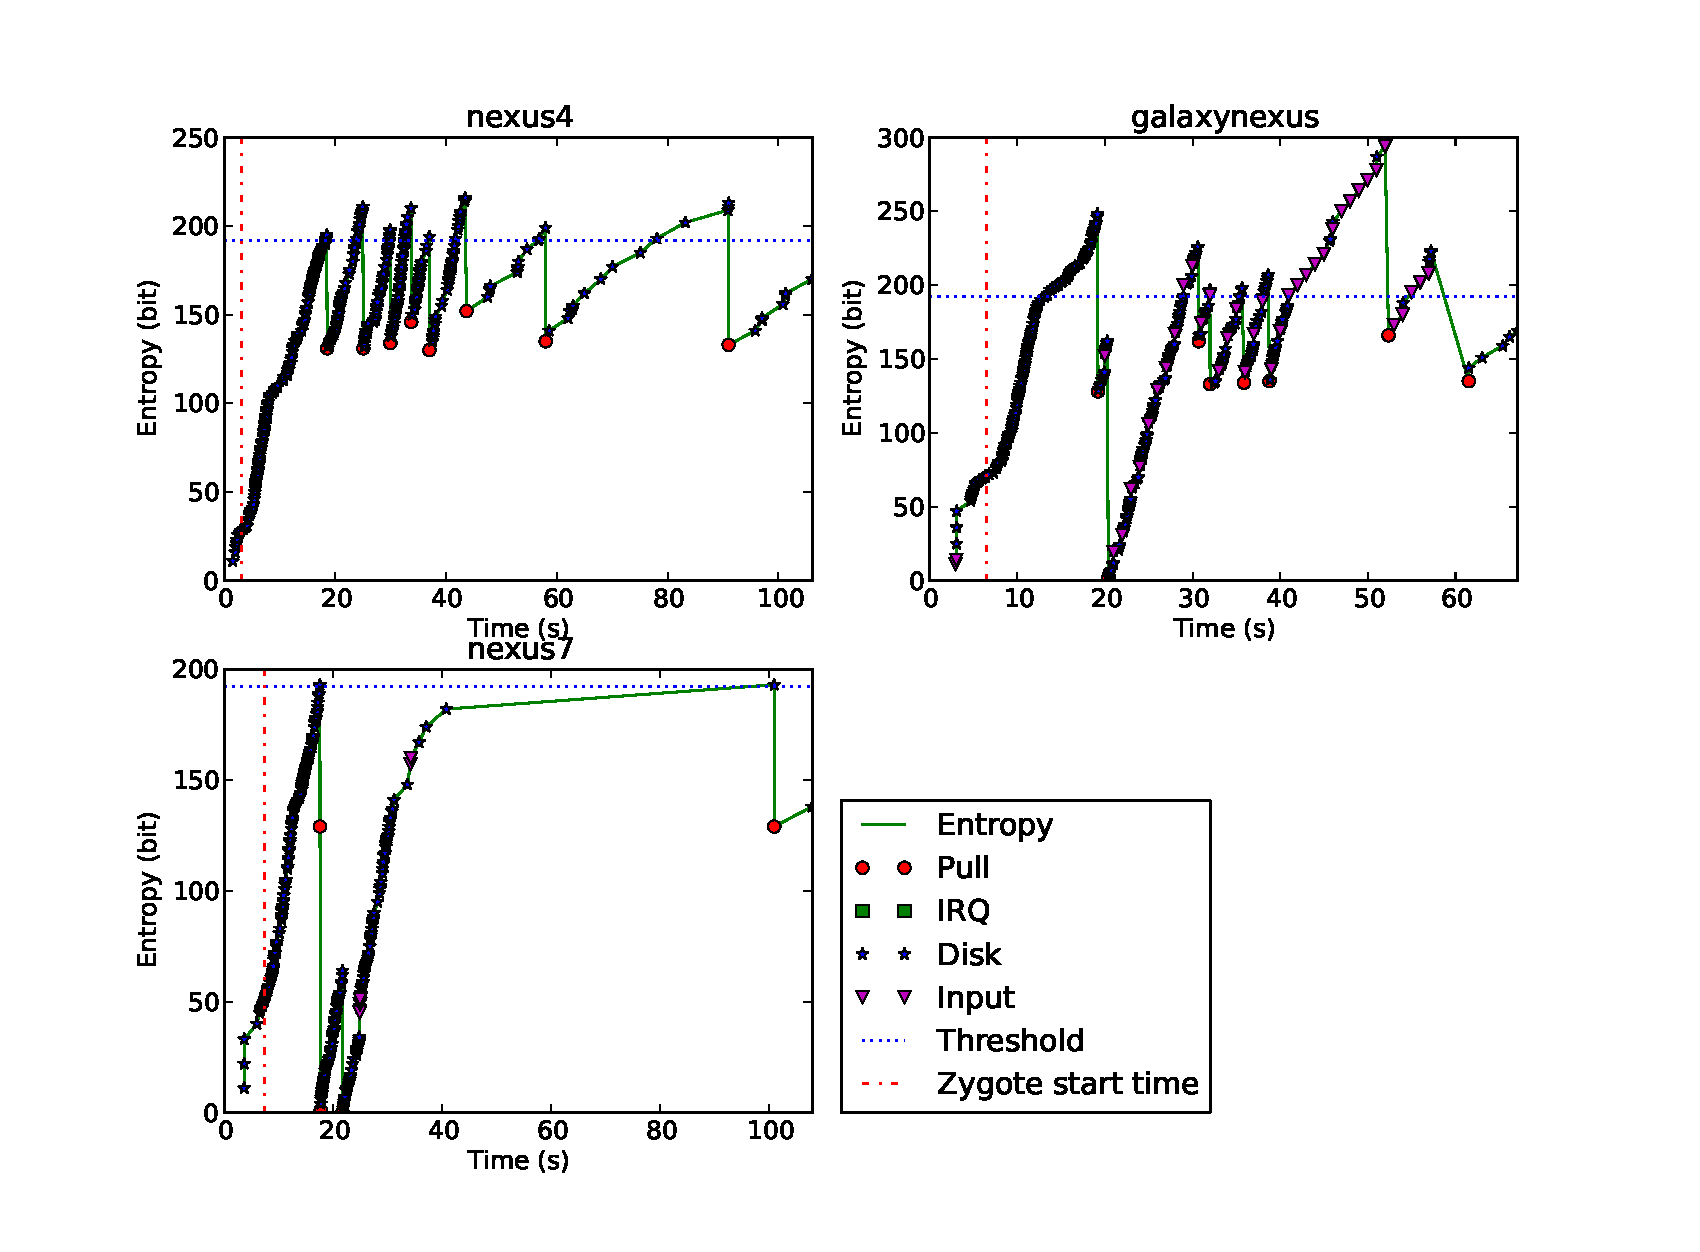
\includegraphics[scale=0.6]{entropy.eps}
\end{center}
\caption{{\bf Amount of Entropy Over Time:} The three devices shows different profiles on entropy accumulation, but their entropy crosses the 192 threshold quickly enough before the user interface is load up. Also note that when Zygote starts the entropy does not cross 192, thus no entropy is mixed into \texttt{/dev/urandom}   }
\label{figentropy}
\end{figure*}

\begin{table}
\begin{center}
\begin{tabular}{|l|c|}
\hline
\bf Device & \bf Full Boot Time (s) \\
\hline
Nexus 4 & ?? \\
\hline
Nexus 7 & 24.8 \\
\hline
Galaxy Nexus & ??\\
\hline

\end{tabular}
\end{center}
\caption{{\bf Full Boot Time:} The time it takes from the kernel is loaded to the Android desktop launcher is brought up.}
\label{tblboottime}
\end{table}

Figure \ref{figentropy} suggests that the Android devices have sufficient source of entropy. The entropy contributed merely by disk events is enough to have \verb|/dev/urandom| properly seeded before any user applications can run.


\subsubsection{User Applications}

Figure \ref{figentropy} and \ref{tblboottime} show that the time when the user could start the first application is after the time when the amount of entropy first crossed the 192 threshold, which means the first read from \verb|/dev/urandom| will cause the non-blocking pool extract at least 10 bytes (\verb|EXTRACT_SIZE| defined in random.c). The 80 bits entropy is enough to prevent any attacker trying to predict the random number. There will be more entropy mixed in when user touches or slides on the screen as shown in table 3. If it is the first boot, users will be asked to setup the wireless network and enter Google account information, which cause a lot of input events and further secure the \verb|/dev/urandom| device. 

Therefore we claim that the user applications are able to enjoy high quality random numbers from the beginning.

\subsubsection{Saving and Restoring the Random Seed}

Android framework has a system service named EntropyMixer which replaces the traditional init script to restore the random seed at boot. There are two major differences between them that may cause security issue:

\begin{itemize}

\item EntropyMixer is an Android service which starts after the Android framework is initialized. Any processes starting before are not protected by the saved entropy. \verb|/dev/urandom| is merely seeded by the time of boot and machine information before that.

\item EntropyMixer reads \verb|/dev/urandom| to save the random seed on boot and then saves every 3 hours instead of before rebooting or halting. This may be a better choice since cell phones are not likely to reboot or halt normally, but it also means the amount of entropy of the saved seed is less than or equal to the amount of entropy of the time of first boot, if the device is rebooted within three hours of its first boot. 

\end{itemize}

\subsubsection{Shared Stack Canary}


\begin{figure}[t]
\begin{center}
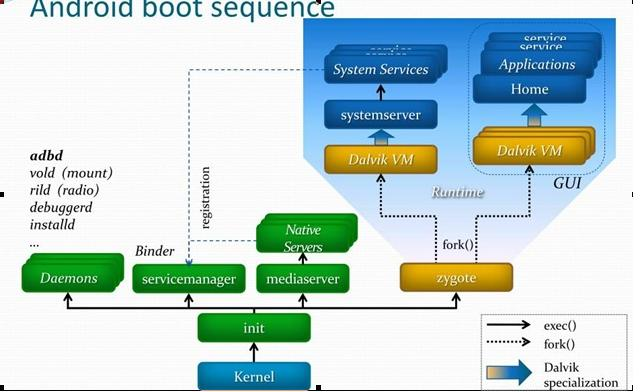
\includegraphics[natwidth=640mm,natheight=392,scale=.3]{bootseq.png}
\end{center}
\caption{{\bf Android boot sequence}} 
\label{figzygote}
\end{figure}



We found that virtually all processes need to read from \verb|/dev/urandom| at their start. We looked into why and found that recent Android versions since 4.0 adopted the stack protector mechanism, as known as stack canaries to protect the Android framework processes as well as native code bridged by Java Native Interface in user applications.

The stack protector works with the help of two components:
\begin{itemize}

\item Android NDK compiler (gcc): insert putting and checking code in function prologues and epilogues. The canary value is read from a global variable.
\item The standard C library (bionic): initialize the canary value by reading 4 bytes from \verb|/dev/urandom| and put it in a global variable. The initialization routine is a library constructor which is invoked by the dynamic linker after mapping the shared library into the process? memory space, typically when the process is exec()ed.
\end{itemize}

However, the way in which the canary value is initialized could be problematic on Android platform. All system services and user applications running on the Dalvik VM are forked from a process called Zygote. By leveraging the Copy-on-Write fork on Linux, Android apps do not need to load the Dalvik VM execution image or the shared library repeatedly on start, leading to better performance. But it also means that there is no chance for an app to invoke the library constructor which setup the canary value. Therefore all Android processes share one stack canary.

We made an app \cite{jnioverflow} to show its canary value on the screen and compared this value to what \verb|app_process| (which then forked Zygote) read from \verb|/dev/urandom| on its start. The result verified this vulnerability. 

\subsubsection{Predictable Stack Canary}

Combining section 2.2 and 2.3, we found that it is possible to predict the canary value shared by all Android apps and Zygote. Note that EntropyMixer is also a system service running on Dalvik VM and thus is going to be forked from Zygote. Therefore, when Zygote sets up its canary value, the \verb|/dev/urandom| is only initialized by its internal routine (\verb|std_initialise|)  with the system information and boot time.

However in our experiment, we found the canary value was not a constant when the initial state of \verb|/dev/urandom| pool was fixed. 

We conjectured that it was due to multitasking and different scheduling realization, because \verb|/dev/urandom| adopts a fine grained locking scheme that maximizes parallelism. It is possible that the internal state changes during the current reading process is descheduled. To verify our conjecture, we modified the \verb|/dev/urandom| interface to enforce a coarse grained locking scheme so that other process cannot change the internal state before the current process finishing reading. It then showed a fixed canary value that depend only on the initial state of \verb|/dev/urandom|.

Given no entropy mixed into the pool of \verb|/dev/urandom|, the internal state depends only on the number of extractions from the pool (this is different from the number of bytes read from \verb|/dev/urandom|, because the minimum number of bytes to extract is 10). With the non-determinism of scheduling, we can model the canary value as a function $f(B,N)$ where $B$ is the boot time and $N$ is the number of extractions from \verb|/dev/urandom| that happened before Zygote read from it.


$B$ is acquired by \verb|getnstimeofday()| function which supports resolution of nanosecond, but we observed only microsecond precision on our devices.
$B$ may not confirm to a specific distribution and the attacker may have knowledge about it in various degrees, we can only make some simple assumption, for example, we can assume that the attacker knows the boot time with precision of second, then the attacker has to guess the microsecond out of $10^6$ values, equivalent to 20 bits of entropy.

$N$ may confirm to some distribution because it can be seen as a value affected by a set of independent events. In order to characterize its distribution, we collected its realization from 244 times of boot; the result is shown in figure \ref{fighist}.

\begin{figure}[t]
\begin{center}
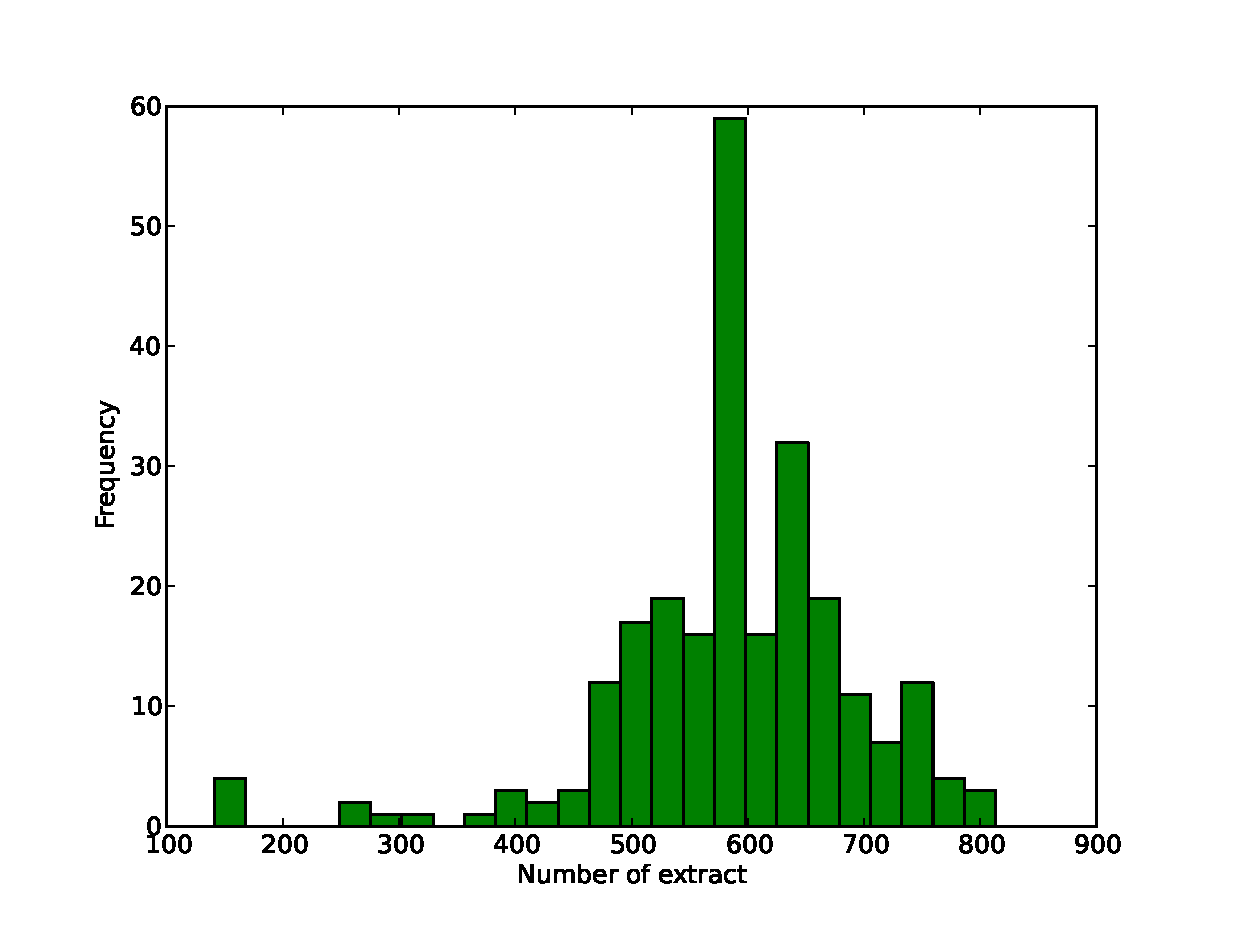
\includegraphics[scale=0.4]{hist.eps}
\end{center}
\caption{{\bf Histogram of number of extractions from \texttt{/dev/urandom} before Zygote runs:} we repeatedly reboot a Nexus 7 for 244 times to record the number of extractions. The result suggests a bell curve distribution of the data which could help the attacker guess the canary value more effciently }
\label{fighist}
\end{figure}

If the attacker has prior knowledge of this distribution of the number of extractions before, he could guess the ranges in a higher probability first order, which gives an expected number of guess of 133 in our case, equivalent to about 7 bits of entropy.

%XXX Entropy estimation!!

With the above model, we can estimate that $B$ and $N$ together will provide 27 bits of entropy, assuming the attacker knows the boot time in second.

Although the computation needed to predict the value of canary may be comparable to simply guessing the 32-bit canary, this vulnerability nullifies the additional security brought by extending the length of the canary. Furthermore, the system time is not a secret number and can be leaked via various ways.

\subsubsection{Nullified ASLR}

Since 4.0, Android has turned on address space layout randomization with the support of the kernel. Despite of only 8 bits of entropy is added for each mapped region, due to the fork nature of Zygote, all Android apps share one address layout, including the same base addresses of the stack, the heap and the standard C library.



\section{Effect and Possible Attacks and Defense}

The sharing values and predictable canary vulnerability affects the following:
\begin{enumerate}

\item All Android applications using NDK: the simplest stack overflow attacks are made possible.

\item Dalvik VM: any buffer overflow vulnerability in DVM can be exploited with only weak defense mechanism.

\item Zygote: similar to 2), but Zygote runs as root and thus is more profitable to exploit.

\end{enumerate}

\subsection{Possible Attacks}

\paragraph*{Possible Attack 1 (side channel / canary collector)} 

As all applications are sharing the stack canary and the base addresses and these values do not change until the next boot, a malicious application could read these values and use them to build payload to overflow other apps running on the device. We made an example of such an attack \cite{jnioverflow}. The malicious application could also collect these values and send to a server. If any buffer overflow vulnerability is found on a popular application, the attacker could compromise many devices as there is no stack protecting mechanism.

\paragraph*{Possible Attack 2: guessing canary} 

Depending on the resolution of the hardware timer and the knowledge the attacker has,  guessing the input of function $f(B, N)$ may take less time than simply guessing the canary value.

\paragraph*{Possible Attack 3: heap overflow}

Heap overflow vulnerabilities are more dangerous because it can circumvent overwriting the canary. A possible heap overflow attack only need to guess 16 bits, including the base addresses of the stack and the heap.

\subsection{Defense}

It is relatively easy to address the predictable canary issue by having Zygote write a new value into the global variable holding the canary after forking a new instance of Dalvik VM. This may bring an overhead of one page of memory due to modification on a CoW page.

The weak ASLR protection is rather hard to fix because:
\begin{itemize}
\item The shared base addresses is due to fork implementation. The Android developers choose to only \verb|fork| instead of \verb|exec| after \verb|fork| to avoid repeatedly mapping same files in to the new process' address space, for all Android apps runs on Dalvik VM and thus need a same set of shared libraries. There seems to be no better way to achieve different address layouts for each forked applications without sacrificing the performance.

\item The weak protection provided by ASLR is due to the 32-bit architecture. It is hard to provide enough entropy that is preventive for attackers to guess with brute force without great modification to the Linux kernel. 

\end{itemize}



\section{Conclusion}

We have investigated the low entropy issue on Android and shown that the poor performance is not caused by blocking reads to /dev/random, since there are none of them. Starting from this issue, we also have investigated possible security vulnerabilities and we have shown that the PRNGs on Android devices are provide secure pseudorandom numbers for all user applications that requires them, because the entropy generated during boot is enough to seed the PRNG properly. However we have found that the stack protecting mechanism initializes the canary value shared by all future Android applications by a value read from the PRNG at an early time when the PRNG is not ready. We have shown that this vulnerability could result in less computation for guessing the canary value, depending on the knowledge of the attacker on the boot time. Furthermore, we have also shown that the shared values vulnerability could leak not only the canary value but the base addresses information, effectively rendering the address space layout randomization mechanism on Android. We have discussed possible attacks against this vulnerability and implemented on of them. In the end, we have proposed a fix to the shared canary vulnerability and argued that the general shared values vulnerability is difficult to fix.
We look into the issue that the amount of entropy kept by the pseudorandom number generator (PRNG) of Android is constantly low. We find that the accusation against this issue of causing poor performance and low frame rate experienced by users is ungrounded. We also investigate possible security vulnerabilities resulting from this issue. We find that this issue does not affect the quality of random numbers that are generated by the PRNG and used in Android applications because recent Android devices do not lack entropy sources. However, we identify a vulnerability in which the stack canary for all future Android applications is generated earlier than the PRNG is properly setup. This vulnerbility makes stack overflow simpler and threats Android applications linked with native code (through NDK) as well as Dalvik VM instances. An attacker could nullify the stack protecting mechanism, given the knowledge of the time of boot or a malicious app running on the victim device. This vulnerability also affects the address space layout randomization (ALSR) mechanism on Android, and can turn it from a weak protection to void. We discuss in this paper several possiable attacks against this vulnerbility as well as ways of defending. As this vulnerbility is rooted in an essential Android design choice since the very first beginning, it is difficult to fix.



%Some embedded literal typset code might 
%look like the following :
%
%{\tt \small
%\begin{verbatim}
%int wrap_fact(ClientData clientData,
%              Tcl_Interp *interp,
%              int argc, char *argv[]) {
%    int result;
%    int arg0;
%    if (argc != 2) {
%        interp->result = "wrong # args";
%        return TCL_ERROR;
%    }
%    arg0 = atoi(argv[1]);
%    result = fact(arg0);
%    sprintf(interp->result,"%d",result);
%    return TCL_OK;
%}
%\end{verbatim}
%}
%
%Now we're going to cite somebody.  Watch for the cite tag.
%Here it comes~\cite{Chaum1981,Diffie1976}.  The tilde character (\~{})
%in the source means a non-breaking space.  This way, your reference will
%always be attached to the word that preceded it, instead of going to the
%next line.
%
%\section{This Section has SubSections}
%\subsection{First SubSection}
%
%Here's a typical figure reference.  The figure is centered at the
%top of the column.  It's scaled.  It's explicitly placed.  You'll
%have to tweak the numbers to get what you want.\\
%
%% you can also use the wonderful epsfig package...
%\begin{figure}[t]
%\begin{center}
%\begin{picture}(300,150)(0,200)
%\put(-15,-30){\special{psfile = fig1.ps hscale = 50 vscale = 50}}
%\end{picture}\\
%\end{center}
%\caption{Wonderful Flowchart}
%\end{figure}
%
%This text came after the figure, so we'll casually refer to Figure 1
%as we go on our merry way.
%
%\subsection{New Subsection}
%
%It can get tricky typesetting Tcl and C code in LaTeX because they share
%a lot of mystical feelings about certain magic characters.  You
%will have to do a lot of escaping to typeset curly braces and percent
%signs, for example, like this:
%``The {\tt \%module} directive
%sets the name of the initialization function.  This is optional, but is
%recommended if building a Tcl 7.5 module.
%Everything inside the {\tt \%\{, \%\}}
%block is copied directly into the output. allowing the inclusion of
%header files and additional C code." \\
%
%Sometimes you want to really call attention to a piece of text.  You
%can center it in the column like this:
%\begin{center}
%{\tt \_1008e614\_Vector\_p}
%\end{center}
%and people will really notice it.\\
%
%\noindent
%The noindent at the start of this paragraph makes it clear that it's
%a continuation of the preceding text, not a new para in its own right.
%
%
%Now this is an ingenious way to get a forced space.
%{\tt Real~$*$} and {\tt double~$*$} are equivalent. 
%
%Now here is another way to call attention to a line of code, but instead
%of centering it, we noindent and bold it.\\
%
%\noindent
%{\bf \tt size\_t : fread ptr size nobj stream } \\
%
%And here we have made an indented para like a definition tag (dt)
%in HTML.  You don't need a surrounding list macro pair.
%\begin{itemize}
%\item[]  {\tt fread} reads from {\tt stream} into the array {\tt ptr} at
%most {\tt nobj} objects of size {\tt size}.   {\tt fread} returns
%the number of objects read. 
%\end{itemize}
%This concludes the definitions tag.
%
%\subsection{How to Build Your Paper}
%
%You have to run {\tt latex} once to prepare your references for
%munging.  Then run {\tt bibtex} to build your bibliography metadata.
%Then run {\tt latex} twice to ensure all references have been resolved.
%If your source file is called {\tt usenixTemplate.tex} and your {\tt
%  bibtex} file is called {\tt usenixTemplate.bib}, here's what you do:
%{\tt \small
%\begin{verbatim}
%latex usenixTemplate
%bibtex usenixTemplate
%latex usenixTemplate
%latex usenixTemplate
%\end{verbatim}
%}
%
%
%\subsection{Last SubSection}
%
%Well, it's getting boring isn't it.  This is the last subsection
%before we wrap it up.
%
%\section{Acknowledgments}
%
%A polite author always includes acknowledgments.  Thank everyone,
%especially those who funded the work. 
%
%\section{Availability}
%
%It's great when this section says that MyWonderfulApp is free software, 
%available via anonymous FTP from
%
%\begin{center}
%{\tt ftp.site.dom/pub/myname/Wonderful}\\
%\end{center}
%
%Also, it's even greater when you can write that information is also 
%available on the Wonderful homepage at 
%
%\begin{center}
%{\tt http://www.site.dom/\~{}myname/SWIG}
%\end{center}
%
%Now we get serious and fill in those references.  Remember you will
%have to run latex twice on the document in order to resolve those
%cite tags you met earlier.  This is where they get resolved.
%We've preserved some real ones in addition to the template-speak.
%After the bibliography you are DONE.

{\footnotesize \bibliographystyle{acm}
\bibliography{../common/bibliography}}


%\theendnotes

\end{document}







